%-----------------------------------------------------------------------------%
\chapter{\babTiga}
%-----------------------------------------------------------------------------%

%-----------------------------------------------------------------------------%
\section{Desain Penelitian}
%-----------------------------------------------------------------------------%
Penelitian ini menggunakan pendekatan eksperimental untuk mengevaluasi efektivitas dan dampak code virtualization menggunakan VxLang. Dua percobaan utama akan dilakukan:

\begin{enumerate}
	\item \bo{Pengujian Autentikasi - Analisis Statis dan Dinamis:} Percobaan ini bertujuan untuk menganalisis kompleksitas control flow program sebelum dan sesudah di-obfuscate menggunakan VxLang. Analisis dilakukan melalui dua pendekatan: analisis statis menggunakan Ghidra dan analisis dinamis menggunakan x64Dbg. Selain itu, percobaan ini juga akan mencakup upaya untuk melewati pengujian autentikasi dengan memanipulasi control flow menggunakan Ghidra dan x64dbg.
	\item \bo{Pengujian Performa - Waktu Eksekusi dan Ukuran File:} Percobaan ini bertujuan untuk mengukur performa waktu eksekusi program dengan algoritma sorting sebelum dan sesudah di-obfuscate, serta membandingkan ukuran file executable. Waktu eksekusi diukur menggunakan library chrono::high\_resolution\_clock.
\end{enumerate}
%-----------------------------------------------------------------------------%
\section{Alat dan Bahan}
%-----------------------------------------------------------------------------%
Perangkat lunak dan perangkat keras yang digunakan dalam penelitian ini adalah:

\begin{itemize}
	\item \bo{Perangkat Lunak:}
	      \begin{itemize}
		      \item \bo{Sistem Operasi:} Windows 11 akan digunakan sebagai lingkungan operasi utama untuk melakukan semua percobaan.
		      \item \bo{Kompiler:} Kompiler Clang (clang-cl) akan digunakan untuk mengkompilasi kode sumber
		      \item \bo{Alat Virtualisasi Kode:} VxLang akan digunakan sebagai alat utama untuk mengimplementasikan virtualisasi kode.
		      \item \bo{Alat Analisis Statis:} Ghidra, sebuah framework reverse engineering yang dikembangkan oleh NSA, akan digunakan untuk melakukan analisis statis.
		      \item \bo{Alat Analisis Dinamis:} x64dbg, sebuah debugger sumber terbuka untuk Windows, akan digunakan untuk analisis dinamis
		      \item \bo{Pustaka C++:} Pustaka chrono akan digunakan untuk mengukur waktu eksekusi dan OpenSSL untuk melakukan enkripsi AES.
	      \end{itemize}
	\item \bo{Perangkat Lunak:}
	      \begin{itemize}
		      \item \bo{Prosesor:} Intel Core i7-12700H
		      \item \bo{RAM:} 32 GB
	      \end{itemize}
\end{itemize}

%-----------------------------------------------------------------------------%
\section{Prosedur Penelitian}
%-----------------------------------------------------------------------------%
\subsection{Pengujian Autentikasi: Analisis Statis dan Dinamis}
Pengujian autentikasi bertujuan untuk mengevaluasi efektivitas virtualisasi kode dalam menghambat upaya reverse engineering dengan menganalisis aspek statis dan dinamis dari perangkat lunak sebelum dan sesudah obfuscation, serta mencoba untuk melewati mekanisme autentikasi.

Berikut persiapan yang akan dilakukan :
\begin{enumerate}
	\item \bo{Pengaturan Lingkungan:} Lingkungan perangkat lunak diatur untuk memastikan bahwa semua alat (Windows 11, Clang, VxLang, Ghidra, dan x64dbg) terinstal dan terkonfigurasi dengan benar. Kode sumber aplikasi studi kasus disiapkan untuk kompilasi.
	\item \bo{Kompilasi Aplikasi Asli:} Aplikasi studi kasus dikompilasi tanpa menerapkan teknik obfuscation apa pun menggunakan kompiler Clang. Hasilnya adalah file executable asli.
	\item \bo{Kompilasi Aplikasi yang di-Obfuscate:} Kode sumber aplikasi studi kasus dimodifikasi untuk menyertakan penanda VL\_VIRTUALIZATION\_BEGIN dan VL\_VIRTUALIZATION\_END untuk menunjukkan blok kode yang akan divirtualisasikan. Kode sumber yang dimodifikasi dikompilasi dengan kompiler Clang, dan selanjutnya, executable diproses dengan VxLang untuk menghasilkan versi yang di-obfuscate yang menyertakan mesin virtual dan bytecode yang sesuai.
\end{enumerate}

\begin{figure}
	\centering
	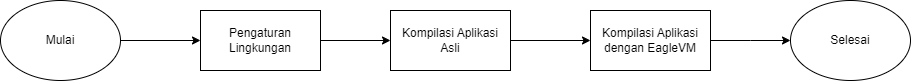
\includegraphics[width=1\textwidth]
	{assets/pics/Persiapan.png}
	\caption{Flow Diagram Persiapan Penelitian}
\end{figure}

\subsubsection{Analisis Statis (Ghidra)}
Fase ini bertujuan untuk menganalisis struktur dan kompleksitas kode tanpa menjalankannya.
\begin{enumerate}
	\item \bo{Peluncuran Ghidra:} Framework Ghidra diluncurkan, dan proyek baru dibuat untuk menampung analisis.
	\item \bo{Mengimpor Executable:} Baik file executable asli maupun yang di-obfuscate diimpor ke dalam proyek Ghidra.
	\item \bo{Analisis Fungsi:} Sebuah fungsi target dalam aplikasi dipilih untuk analisis terfokus. Alat analisis Ghidra digunakan untuk membongkar fungsi target dan menghasilkan Control Flow Graph (CFG) untuk kedua versi executable.
	\item \bo{Perbandingan CFG:} CFG dari versi asli dan yang di-obfuscate dibandingkan dengan mendokumentasikan jumlah basic block, edge, dan kompleksitas siklomatik. Kompleksitas siklomatik yang lebih tinggi berkorelasi dengan peningkatan kesulitan dalam pemahaman kode dan reverse engineering. Dokumentasi untuk setiap versi akan mencakup yang berikut:
	      \begin{itemize}
		      \item \bo{Jumlah Basic Block:} Ini menunjukkan jumlah total urutan kode non-percabangan dalam alur kontrol fungsi.
		      \item \bo{Jumlah Edge:} Ini mewakili alur eksekusi dari satu blok ke blok lainnya.
		      \item \bo{Kompleksitas Siklomatik:} Metrik ini mengukur jumlah jalur independen dalam alur kontrol kode. Ini dihitung berdasarkan rumus: Edge - Node + 2
	      \end{itemize}
	\item \bo{Mendokumentasikan Temuan:} Catatan dan observasi terperinci mengenai analisis statis kode dipelihara.
\end{enumerate}

\begin{figure}
	\centering
	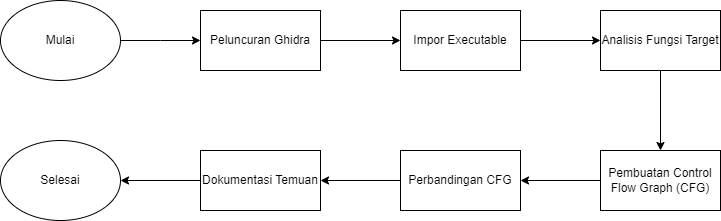
\includegraphics[width=1\textwidth]
	{assets/pics/Static.png}
	\caption{Flow Diagram Analisis Statis}
\end{figure}

\bo{Upaya Manipulasi Control Flow:}
\begin{enumerate}
	\item \bo{Identifikasi Mekanisme Autentikasi:} Menggunakan Ghidra, identifikasi bagian kode yang menangani proses autentikasi. Ini melibatkan pencarian fungsi yang memvalidasi kredensial atau memeriksa lisensi.
	\item \bo{Analisis Control Flow:} Analisis control flow dari fungsi autentikasi untuk memahami bagaimana keputusan autentikasi dibuat.
	\item \bo{Modifikasi Control Flow:} Menggunakan Ghidra, modifikasi kode assembly untuk mengubah alur kendali agar melewati pemeriksaan autentikasi. Ini bisa melibatkan perubahan conditional jump atau patching instruksi.
	\item \bo{Penyimpanan Perubahan:} Setelah modifikasi dilakukan, simpan perubahan pada file executable yang telah di-patch.
	\item \bo{Pengujian:} Jalankan file executable yang telah dimodifikasi dan verifikasi apakah modifikasi control flow berhasil melewati mekanisme autentikasi.
\end{enumerate}

\subsubsection{Analisis Dinamis (x64dbg)}
Analisis dinamis melibatkan pengamatan perilaku program saat dijalankan.
\begin{enumerate}
	\item \bo{Peluncuran x64Dbg:} Debugger x64dbg diluncurkan, dan baik executable asli maupun yang di-obfuscate dimuat.
	\item \bo{Pengaturan Breakpoint:} Breakpoint ditempatkan di awal fungsi target dalam setiap versi aplikasi untuk mengontrol eksekusi selama analisis.
	\item \bo{Menjalankan dan Mengamati:} Aplikasi dijalankan, dan eksekusi dilacak. Ini termasuk mengamati alur eksekusi, perilaku program, dan mencatat setiap perbedaan dalam jalur eksekusi.
	\item \bo{Mendokumentasikan Temuan:} Catatan terperinci dibuat tentang perbedaan yang diamati dalam alur eksekusi dan kesulitan yang dihadapi dalam memahami perilaku versi yang di-obfuscate.
\end{enumerate}

\begin{figure}
	\centering
	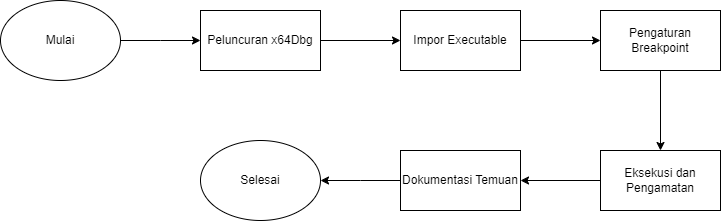
\includegraphics[width=1\textwidth]
	{assets/pics/Dynamic.png}
	\caption{Flow Diagram Analisis Dinamis}
\end{figure}

\subsection{Pengujian Performa: Waktu Eksekusi dan Ukuran File}
Pengujian kinerja ini bertujuan untuk mengevaluasi dampak virtualisasi kode terhadap waktu eksekusi dan ukuran file aplikasi. Untuk mendapatkan pengukuran yang komprehensif, kita akan menggunakan algoritma pengurutan (sorting) sebagai benchmark.

Berikut persiapan yang akan dilakukan :
\begin{enumerate}
	\item \bo{Pemilihan Algoritma Pengurutan:} Algoritma pengurutan yang akan digunakan sebagai benchmark adalah algoritma pengurutan cepat (Quicksort). Quicksort dipilih karena efisiensinya yang baik dalam banyak kasus, serta kompleksitasnya yang cukup untuk memberikan gambaran yang baik tentang performa.
	\item \bo{Pengembangan Benchmark:} Benchmark akan diimplementasikan dengan membuat fungsi yang melakukan pengurutan pada array data. Array data akan diisi dengan angka acak untuk memastikan pengujian yang representatif. Ukuran array data akan divariasikan (misalnya, 1000, 10000, 100000 elemen) untuk mengamati performa pada berbagai skala data.
	\item \bo{Integrasi Benchmark:} Fungsi benchmark diintegrasikan ke dalam kedua versi aplikasi (asli dan yang di-obfuscate). Hal ini memungkinkan kita untuk mengukur waktu eksekusi dari algoritma pengurutan pada kedua versi aplikasi secara terpisah.
\end{enumerate}

\subsubsection{Pengukuran Waktu Eksekusi}
\begin{enumerate}
	\item \bo{Eksekusi Benchmark:} Fungsi benchmark (algoritma pengurutan) akan dieksekusi beberapa kali (misalnya, N=10) pada setiap ukuran array untuk mendapatkan data yang cukup.
	\item \bo{Pengukuran Waktu:} Pustaka chrono::high\_resolution\_clock dari C++ akan digunakan untuk mengukur secara akurat waktu yang dibutuhkan untuk setiap eksekusi benchmark.
	\item \bo{Pencatatan Data:} Waktu eksekusi setiap run (dalam milidetik atau mikrosekon) dicatat untuk setiap ukuran array pada kedua versi aplikasi.
	\item \bo{Perhitungan Rata-Rata:} Waktu eksekusi rata-rata dihitung untuk setiap versi dan setiap ukuran array dengan menjumlahkan semua waktu eksekusi dan membaginya dengan jumlah run (N).
\end{enumerate}

\subsubsection{Pengukuran Ukuran File}
\begin{enumerate}
	\item \bo{Perbandingan Ukuran File:} Ukuran file dari executable asli dan yang di-obfuscate dibandingkan untuk menentukan dampak virtualisasi kode pada ukuran aplikasi.
\end{enumerate}

\begin{figure}
	\centering
	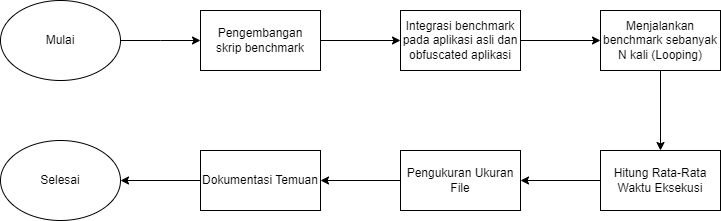
\includegraphics[width=1\textwidth]
	{assets/pics/Performance.png}
	\caption{Flow Diagram Analisis Performa}
\end{figure}

\section{Teknik Analisis Data}
Data yang dikumpulkan dari kedua rangkaian percobaan akan dianalisis menggunakan teknik deskriptif dan komparatif.
\subsection{Analisis Data Pengujian Autentikasi}
\begin{itemize}
	\item \bo{Analisis Data Statis:} Metrik kompleksitas yang diperoleh dari analisis statis (yaitu, jumlah basic block, edge, dan kompleksitas siklomatik) akan dievaluasi. Perbedaan akan digunakan untuk menilai efektivitas virtualisasi kode.
	\item \bo{Analisis Data Dinamis:} Hasil dari analisis dinamis, termasuk alur eksekusi yang diamati dan kesulitan dalam analisis kode, akan dianalisis.
	\item \bo{Evaluasi Efektivitas Keamanan:} Hasil dari analisis dinamis, termasuk alur eksekusi yang diamati dan kesulitan dalam analisis kode, akan dianalisis.
\end{itemize}

\subsection{Analisis Data Pengujian Autentikasi}
\begin{itemize}
	\item \bo{Perbandingan Waktu Eksekusi:} Waktu eksekusi rata-rata antara aplikasi asli dan yang di-obfuscate dibandingkan untuk menilai potensi overhead kinerja yang diperkenalkan oleh VxLang.
	\item \bo{Perbandingan Ukuran File:} Ukuran file dari kedua versi dibandingkan untuk menilai dampak ukuran file dari virtualisasi kode.
	\item \bo{Analisis Trade-off:} Analisis komprehensif dilakukan untuk mengevaluasi trade-off antara keamanan dan kinerja, berdasarkan temuan.
\end{itemize}
